\section{Econometrics Final 2017 / 18}

{
\subsection*{Watson}

{
\subsubsection*{Exercise 1}

\begin{enumerate}[label=(\alph*)]
{\item 
$$
\begin{aligned}
\mathbb{E}_{t}\left(Y_{t+1} \mid \varepsilon_{t}+\varepsilon_{t-1}=2\right) & =\mathbb{E}_{t}\left(\varepsilon_{t+1}+0.8 \varepsilon_{t} \mid \varepsilon_{t}=2-\varepsilon_{t-1}\right) \\
& =\mathbb{E}_{t}\left(\varepsilon_{t+1}+0.8\left(2-\varepsilon_{t-1}\right)\right) \\
& =\mathbb{E}_{t}\left(\varepsilon_{t+1}\right)+1.6-0.8 \mathbb{E}_{t}\left(\varepsilon_{t-1}\right) \\
& =1.6
\end{aligned}
$$

The optimal forecast is the conditional expectation of $Y_{t+1}$ given the information that $\varepsilon_{t}+\varepsilon_{t-1}=2$.
}
{\item 
$$
\begin{aligned}
\hat{\phi} &= \frac{\widehat{\operatorname{Cov}}\left(Y_{t}, Y_{t-1}\right)}{\widehat{\operatorname{Var}}\left(Y_{t-1}\right)} \\
\xrightarrow{p} \frac{\operatorname{Cov}\left(Y_{t}, Y_{t-1}\right)}{\operatorname{Var}\left(Y_{t-1}\right)} & =\frac{\operatorname{Cov}\left(\varepsilon_{t}+0.8 \varepsilon_{t-1}, \varepsilon_{t-1}+0.8 \varepsilon_{t-2}\right)}{\operatorname{Var}\left(\varepsilon_{t-1}+0.8 \varepsilon_{t-2}\right)} \\
& =\frac{\operatorname{Var}\left(\varepsilon_{t-1}\right) \cdot 0.8}{\operatorname{Var}\left(\varepsilon_{t-1}\right)+0.64 \operatorname{Var}\left(\varepsilon_{t-2}\right)} \\
& =\frac{0.8}{1.64}=0.488
\end{aligned}
$$
}
\end{enumerate}
}
{
\subsubsection*{Exercise 2}

\begin{enumerate}[label=(\alph*)]
{\item 
It is not invertible. Let $X_{t}=Y_{t}-\beta$, then

$$
\begin{aligned}
X_{t} & =\varepsilon_{t}-\theta \varepsilon_{t-1} \\
\Leftrightarrow \varepsilon_{t} & =X_{t}+\theta \varepsilon_{t-1} \\
& =X_{t}+\theta\left(X_{t-1}+\theta \varepsilon_{t-2}\right) \\
& \quad \vdots \\
& =\theta^{t} \varepsilon_{0}+\sum_{i=0}^{t-1} \theta^{i} X_{t-i}
\end{aligned}
$$

If $|\theta| \geq 1$, then $\theta^{t} \varepsilon_{0}$ does not converge towards zero as $t$ gets large. Therefore, $X_{t}$ cannot be expressed only by its lagged values plus the period $t$ error.
}
{\item 
$$
\begin{aligned}
\sqrt{T}(\bar{Y}-\beta) & =\sqrt{T} \frac{1}{T} \sum_{t=1}^{T}\left(Y_{t}-\beta\right)=\frac{1}{\sqrt{T}} \sum_{t=1}^{T}\left(\varepsilon_{t}-\theta \varepsilon_{t-1}\right) \\
& =\frac{1}{\sqrt{T}}\left(\sum_{t=1}^{T} \varepsilon_{t}-\theta \sum_{t=0}^{T-1} \varepsilon_{t}\right)
\end{aligned}
$$

$$
\begin{aligned}
& =\frac{1}{\sqrt{T}}\left(\sum_{t=1}^{T} \varepsilon_{t}-\theta \sum_{t=1}^{T} \varepsilon_{t}-\theta \varepsilon_{0}+\theta \varepsilon_{T}\right) \\
& =\underbrace{(1-\theta) \frac{1}{\sqrt{T}} \sum_{t=1}^{T} \varepsilon_{t}}_{\xrightarrow{d} N(0,\sigma^2(1-\theta)^2)}+\underbrace{\frac{\theta}{\sqrt{T}}\left(\varepsilon_{T}-\varepsilon_{0}\right)}_{\xrightarrow{p}0}
\end{aligned}
$$

Apply Slutsky:

$$
\begin{aligned}
& \sqrt{T}(\bar{Y}-\beta) \xrightarrow{d} N\left(0, \sigma^{2}(1-\theta)^{2}\right) \\
& \sqrt{T}(\bar{Y}-\beta) \xrightarrow{d} N(0,1)
\end{aligned}
$$
}
{\item 
Delta method: $g(x)=x^{2} ;\left(g^{\prime}(x)\right)^{2}=4 x^{2}$

$$
\sqrt{T}\left(\bar{Y}^{2}-\beta^{2}\right) \xrightarrow{d} N\left(0,1 \cdot g^{\prime}(\beta)^{2}\right)
$$

Use $g^{\prime}(\beta)^{2}=4 \beta^{2}$ and $\beta=5$. Then:

$$
\sqrt{T}\left(\bar{Y}^{2}-25\right) \xrightarrow{d} N\left(0,100\right)
$$
}
{\item 
If $\theta=1$, this would lead to $V=0$ which is clearly incorrect. There, I would do the following:

$$
\begin{aligned}
Y_{t}-\beta & =u_{t}=\varepsilon_{t}-\varepsilon_{t-1} \\
\frac{1}{\sqrt{T}} \sum Y_{t}-\beta & =\frac{1}{\sqrt{T}} \sum_{t=1}^{T} u_{t}
\end{aligned}
$$

Now $u_{t} \sim N(0,2)$ but not iid anymore.

\color{red} How further?? \color{black}
}
\end{enumerate}
}
{
\subsubsection*{Exercise 3}

\begin{enumerate}[label=(\alph*)]
{\item 
$$
\begin{aligned}
& \bar{X}_{t}=\frac{1}{n} \sum_{i=1}^{n} \xi_{t}+\varepsilon_{i t}=\xi_{t}+\frac{1}{n} \sum_{i=1}^{n} \varepsilon_{i t} \\
& \xi_{t} \xrightarrow{p} \xi_{t} \text { as } \xi_{t}=\xi_{t} \\
& \frac{1}{n} \sum_{i=1}^{n} \varepsilon_{t} \xrightarrow{p} \mathbb{E}\left(\varepsilon_{i t}\right)=0 \text { by LLN}
\end{aligned}
$$

I conclude that

$$
\bar{X}_{t} \longrightarrow \xi_{t}
$$
}
{\item 
$$
\begin{aligned}
M S E & =\mathbb{E}\left(\left(\bar{X}_{t}-\xi_{t}\right)^{2}\right) \\
& =\mathbb{E}\left(\left(\frac{1}{n} \sum_{i=1}^n \varepsilon_{i t}\right)^{2}\right)=\left(\frac{1}{n}\right)^{2} \mathbb{E}\left(\sum_{i=1}^{n} \varepsilon_{i t}^{2}+\sum_{j \neq i} \varepsilon_{i t} \varepsilon_{j t}\right) \\
& =\frac{1}{n^{2}} \sum_{i=1}^{n} \underbrace{\mathbb{E}\left(\varepsilon_{it}^{2}\right)}_{\sigma^{2}=1}+\sum_{j \neq i} \underbrace{\mathbb{E}\left(\varepsilon_{i t} \varepsilon_{j t}\right)}_{=0 \text { by iid } N(0,1)} \\
& =\frac{1}{n}
\end{aligned}
$$
}
{\item 
\color{red} Maybe MLE-estimator? \color{black}
}
\end{enumerate}
}
}

\newpage
{
\subsection*{Honor\'e}

{
\subsubsection*{Exercise 1}

\begin{enumerate}[label=(\alph*)]
{\item 
$C I=[\hat{\beta} \pm 1.96 \cdot \hat{SE}(\hat{\beta})] \cong[0.227 ; 0.962]$
}
{\item 
Reject the hypothesis:

$$t=\frac{\hat{\beta}-\beta_{0}}{\hat{SE}(\hat{\beta})}=\frac{0.092+0.2}{0.115}=2.545>1.96$$
}
{\item 
$$
\begin{aligned}
x_{i}^{\prime} \beta & =1.1 \cdot 0.98+0.8 \cdot 0.152+1 \cdot(-0.223)-1.872 \\
& =-0.896 \\
P\left(y_{i} =1 | x_{i}\right)&=\frac{\exp \left(x_{i}^{\prime} \beta\right)}{1+\exp \left(x_{i}^\prime \beta\right)} \cong 28.993 \%
\end{aligned}
$$
}
{\item 
$$
\begin{aligned}
\frac{\partial P\left(y_{i}=1 \mid x_{i}\right)}{\partial b l o o d p} & =P\left(y_{i}=1 \mid x_{i}\right) P\left(y_{i}=0 \mid x_{i}\right) \cdot \beta_{\text {bloodp }} \\
& \cong 0.202
\end{aligned}
$$
}
\end{enumerate}
}
{
\subsubsection*{Exercise 2}

\begin{enumerate}[label=(\arabic*)]
{\item 
$$
\begin{aligned}
\sqrt{n}(\hat{\beta}-\beta) &\xrightarrow{d} N\left(0, A^{-1} B A^{-1}\right) \\
A &=\mathbb{E}\left(\left(1+2 \beta x_{i}\right)^{2}\right)\\
B &=\sigma^{2} \mathbb{E}\left(\left(1+2 \beta x_{i}\right)^{2}\right)
\end{aligned}
$$

Thus, we can simplify:

$$
\sqrt{n}(\hat{\beta}-\beta) \xrightarrow{d} N\left(0, \sigma^{2} \mathbb{E}\left(\left(1+2 \beta x_{i}\right)^{2}\right)^{-1}\right)
$$
}
{\item 
$$
\begin{aligned}
\sqrt{n}(\hat{\beta}-\beta) &\xrightarrow{d} N\left(0, G^{-1} S G^{-1}\right) \\
G &= \mathbb{E}\left(-x_{i}\left(1+2 \beta x_{i}\right)\right)=-\left(\mathbb{E}\left(x_{i}\right)+2 \beta \mathbb{E}\left(x_{i}^{2}\right)\right) \\
S &= V\left(\left(y_{i}-\left(\beta+\beta^{2} x_{i}\right)\right) x_{i}\right)=V\left(\varepsilon_{i} x_{i}\right) \\
&= \mathbb{E}\left(\varepsilon_{i}^{2} x_{i}^{2}\right)-\mathbb{E}\left(\varepsilon_{i} x_{i}\right)^{2}=\mathbb{E}\left(\mathbb{E}\left(\varepsilon_{i}^{2} \mid x_{i}\right) x_{i}^{2}\right) \\
&= \sigma^{2} \mathbb{E}\left(x_{i}^{2}\right)
\end{aligned}
$$
}
{\item 
$$
\begin{aligned}
& \sqrt{n}(\hat{\beta}-\beta) \xrightarrow{d} N\left(0, \left(G^{\prime} S^{-1} G\right)^{-1}\right) \\
& G=\mathbb{E}\left[\begin{array}{l}
-\left(1+2 \beta x_{i}\right) \\
-x_{i}\left(1+2 \beta x_{i}\right)
\end{array}\right] \\
& S=V\left[\begin{array}{ll}
\varepsilon_{i} \\
\varepsilon_{i} x_{i}
\end{array}\right]=\mathbb{E}\left[\begin{array}{ll}
\varepsilon_{i}^{2} & \varepsilon_i^{2} x_{i} \\
\varepsilon_{i}^{2} x_{i} & \varepsilon_{i}^{2} x_{i}^{2}
\end{array}\right]=\sigma^{2}\left[\begin{array}{ll}
1 & \mathbb{E}\left(x_{i}\right) \\
\mathbb{E}\left(x_{i}\right) & \mathbb{E}\left(x_{i}^{2}\right)
\end{array}\right]
\end{aligned}
$$
}
\end{enumerate}
}
{
\subsubsection*{Exercise 3}

\begin{itemize}
\item When we think that the treatment is that some variable $x$ is greater then some threshold $c$. Examples would be:
\begin{itemize}
    \item let $x$ be time, $c$ be the year 1989, and $y$ is GDP growth in eastern Germany. Since before $c$, eastern Germany was under communist rule, one could interpret 1989 as the threshold after which the treatment "capitalism" was implemented.
    \item let $x$ be school grades, $c$ be the cutoff to get into med-school, and $y$ be earnings. We can use this cut-off as a treatment.
\end{itemize}
\item It assumes, that the regressions in the counterfactual would continue continuously. Also, that the treatment at $c$ actually causes a jump in $y$.
\end{itemize}

The following graph helps to drive the idea home:

\begin{figure}[!htp]
    \centering
    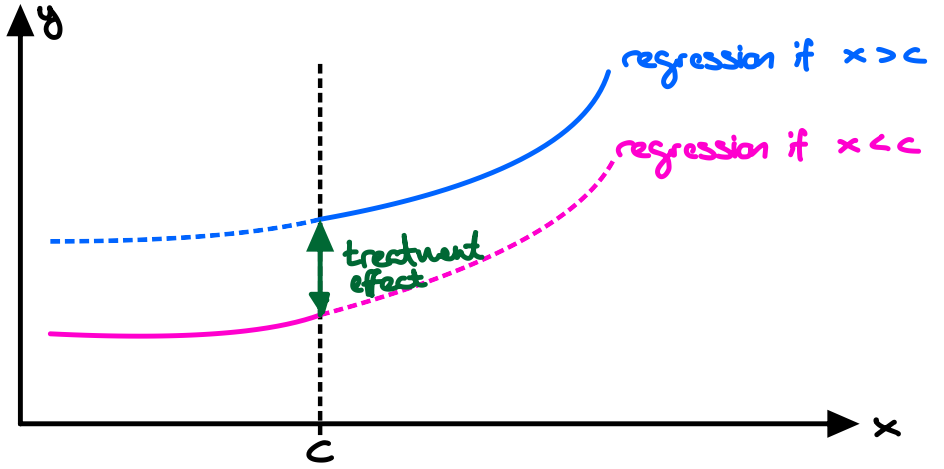
\includegraphics[width=\textwidth]{images/2017_18.png}
\end{figure}
}
{
\FloatBarrier
\subsubsection*{Exercise 4}

First, we get rid of the $\alpha_{i}$ by taking first differences:

$$
\Delta y_{i t}=\Delta x_{i t} \beta_{1}+\Delta x_{2i t} \beta_{2}+\Delta \varepsilon_{i t} \quad t=2,3
$$

Note, that we can use the following to find the moment conditions:

$$
\begin{aligned}
\mathbb{E}\left(\Delta \varepsilon_{i t} \mid x_{1is}\right)=0 & \quad \forall t,s \\
\mathbb{E}\left(\Delta \varepsilon_{i t} \mid x_{2 i s}\right)=0 & \quad \forall t \geq s
\end{aligned}
$$

$$
\begin{aligned}
\text{for }x_{1 i t}: \quad & \mathbb{E}\left(\Delta \varepsilon_{i t} x_{1 i s}\right)=0 \quad \forall s, t \\
&\mathbb{E}\left(\Delta y_{i t}-\Delta x_{1i t} \beta_{1}+\Delta x_{2 it} \beta_{2}\right) x_{1 i s}=0 \quad \forall s, t \\
&\longrightarrow 6 \text{ moment conditions} \\
\text{for }x_{2 i t}: \quad & \mathbb{E}\left(\Delta \varepsilon_{i t} x_{2is}\right)=0 \quad \forall (s, t) \in\{(1,2),(1,3),(2,3)\} \\
&\mathbb{E}\left(\left(\Delta y_{i t}-\Delta x_{1 i t} \beta_{1}+\Delta x_{2i t} \beta_{2}\right) x_{2 i s}\right)=0 \quad \forall (s, t) \in\{(1,2),(1,3),(2,3)\} \\
&\longrightarrow 3 \text{ moment conditions}
\end{aligned}
$$

Therefore, we can use 9 moment conditions in total, and GMM will work to estimate $\left(\beta_{1}, \beta_{2}\right)$.
}
}
